\chapter{Gestion des variations} % Main chapter title
\label{Chapitre3} % For referencing the chapter elsewhere, use \ref{Chapter1} 
\lhead{Chapitre 3. \emph{Gestion des variations}} % This is for the header on each page - perhaps a shortened title
Une variation est considéré comme toute action non définie dans le modèle de procédé initiale ou qui viole certaines contraintes de procédés.
Après une étude de l'existant, nous allons proposer deux solutions de gestion de variations. La première solution consiste à traiter les variations grâce à un PSEE; la seconde solution quand à elle, utilise un macro pour gérer les variations.
Dans ce chapitre nous présenteront nos techniques de détection de variations (la technique à l'aide d'un PSEE et la seconde technique à l'aide d'un fichier excel) et nos plans de corrections.
\section{Solution 1}
Comme nous l'avons dit dans le chapitre~\ref{Chapitre2}, l'OMG a proposé en 2005 le SPEM 1.1, mais ce dernier (SPEM 1.1) présentant quelques lacunes, ils ont proposé en 2008 une nouvelle version (SPEM 2.2). 
Ces normes de l'OMG sont utilisées dans de nombreux travaux de recherches car elles sont considérées aujourd'hui comme étant des normes assez complètes pour pouvoir décrire les procédés. Alors pour cette première solution, je me suis beaucoup basé sur les solutions proposées par l'OMG dans leurs travaux.
\subsection{Méta-modèle de procédé}
Avant d'expliquer la technique de détection, nous allons définir notre méta-modèle de procédé c'est à dire notre modèle définissant les concepts de base d'un langage de description de procédés.
La figure~\ref{metamodele} représente notre méta-modèle de procédé. Nous avons récupéré les éléments importants proposés par l'OMG et avons rajouter nos éléments pour nous permettre de détecter et de corriger les variations.
\begin{figure}[h]
\centering
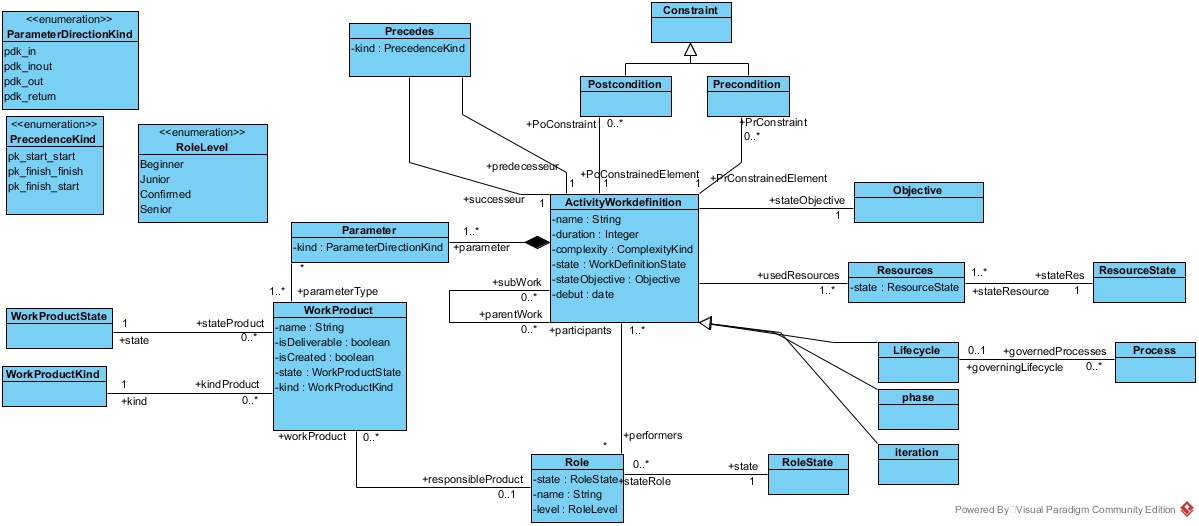
\includegraphics[width=16cm]{Solution.jpg}
\caption{\label{metamodele}Méta-modèle de SPEM solution}
\end{figure}
Nous allons maintenant décrire chaque élément de notre méta-modèle.
\subsubsection*{ActivityWorkDefinition}
L'élément \textbf{\textit{ActivityWorkDefinition}} représente un travail ou une tâche à réaliser durant le processus de développement logiciel. Ces tâches doivent être réalisées par des acteurs décrits par \textit{Role} pendant une durée donnée.\\
Les attributs de cet élément sont:\\
\begin{itemize}
\item[\tiny{$\blacksquare$}] Name: c'est une chaine de caractère qui correspond au nom de la tâche.
\item[\tiny{$\blacksquare$}] State: de type \textit{ActivityWorkDefinitionState}, il permet de connaitre l'état de la tâche.
\item[\tiny{$\blacksquare$}] Duration: nombre représentant la durée de la tâche.
\item[\tiny{$\blacksquare$}] Complexity: indique le niveau de difficulté ou le degré de complexité de la tâche. Il pourra nous être utile pendant le traitement d'une déviation.
\item[\tiny{$\blacksquare$}] stateObjective: attribut de type \textit{Objective}, il indique l'objectif ou le but du travail.
\end{itemize}
\subsubsection*{WorkProduct, WorkProductKind, WorkProductState}
L'élément \textbf{\textit{WorkProduct}} ou artéfact représente tout ce qui est produit, modifié ou consommé par un \textit{ActivityWorkDefinition}. Ses attributs sont:\\
\begin{itemize}
\item[\tiny{$\blacksquare$}] Name: chaine de caractère représentant le nom du produit.
\item[\tiny{$\blacksquare$}] isDeliverable: booléen permettant de savoir si le produit peut être délivré ou pas.
\item[\tiny{$\blacksquare$}] Kind: de type \textit{WorkProductKind}, il permet de connaitre le type du produit c'est à dire si c'est un document, model ou code.
\item[\tiny{$\blacksquare$}] State: indique l'état du produit, il est de type \textit{WorkProductState}.
\item[\tiny{$\blacksquare$}] isCreated: booléen permettant de savoir si le produit fut crée ou pas par la tâche.
\end{itemize}
Un \textbf{\textit{WorkProductKind}} représente les catégories de produits que l'on peut avoir. Ces catégories peuvent être du code, des documents, du model etc.\\
L'élément \textit{WorkProductState} indique les états d'un produit (initial, validé, invalidé etc...)

\subsubsection*{RoleLevel, Role}
\textit{RoleLevel} est une énumération des niveaux qu'un rôle peut avoir (débutant, junior, confirmé, senior).\\
Un \textit{Role} représente les rôles ou acteurs responsables d'un produit ou contribuant à la réalisation d'une tâche. Par exemple on peut avoir des analystes, des testeurs etc... Cet élément rôle possède un attribut \textit{name} qui indique le nom du rôle;  un attribut \textit{state} indiquant l'état du rôle c'est à dire si le rôle a terminé d'accomplir la tâche ou si il est en train de le faire etc... et un attribut \textit{level} qui indique le niveau de l'acteur (débutant, junior, confirmé). 
\subsubsection*{Postcondition et Precondition}
Les éléments \textbf{\textit{Precondition}} et \textbf{\textit{Postcondition}} sont des spécialisation de la classe \textit{Constraint}. Il représentent respectivement les conditions qui doivent être satisfaites avant et après l'exécution de chaque \textit{ActivityWorkDefinition}. 
\subsubsection*{Parameter}
L'élément \textbf{\textit{Parameter}} est composé d'un attribut \textit{kind} de type \textbf{\textit{ParameterDirectionKind}} qui est une énumération des types de relations qui relie une tâche à un produit. C'est à dire qu'il permet d'indiquer si un \textit{WorkProduct} est utilisé par une \textit{ActivityWorkDefinition} tant que \og entrée \fg{}, \og sortie \fg{} ou \og entrée/sortie \fg{}. 
\subsubsection*{Precedes et PrecedenceKind}
Pour expliquer les relations qui lient nos \textit{ActivityWorkDefinition}, nous allons prendre deux tâches t1 et t2, t2 étant le successeur de t1.
L'élément \textbf{\textit{PrecedenceKind}} est une énumération des relations qui peuvent exister entre nos \textit{ActivityWorkDefinition}: 
\textit{pk\_start\_start}: ce type de relation permet d'indiquer que t2 ne pourra commencer que si t1 commence.\\
\textit{pk\_finish\_finish}: ce type de relation permet d'indiquer que t2 ne pourra terminer que si t1 l'est.\\
\textit{pk\_finish\_start}: indique que t2 ne pourra commencer qu'à la fin de t1.\\
L'élément \textbf{\textit{Precedes}} comporte un attribut \textit{kind} de type \textit{PrecedenceKind}, il indique le type d'ordonnancement qui relie les \textit{ActivityWorkDefinition}. Par exemple supposons que nos deux tâches t1 et t2 sont reliées par une liaison de type pk\_start\_start, t2 ne peut pas commencer tant que t1 n'a pas commencé.
\subsubsection*{Objective}
L'élément \textbf{\textit{Objective}} représente l'objectif ou le but de la réalisation d'une tâche. Si une tâche est terminée, on pourra vérifier si l'objectif a été atteint.
\subsubsection*{ResourceState, Resources}
\textit{ResourceState} représente les états de disponibilités des ressources.
L'élément \textbf{\textit{Ressources}} représente les différentes ressources. Ces ressources sont utilisées par des tâches selon leurs disponibilités.
\subsubsection*{LifeCycle, Phase, Iteration}
L'élément \textbf{\textit{LifeCycle}} représente le cycle de vie de logiciel par exemple\og le modèle cascade \fg{} ou\og le modèle en V\fg{}
La \textbf{\textit{Phase}} est une spécialisation de \textit{ActivityWorkDefinition}. C'est une tâche correspondant à une phase d'un cycle de vie de logiciel 
L'élément \textbf{\textit{Iteration}} est une \textit{ActivityWorkDefinition} avec des préconditions et objectif bien défini appelé \og minor milestone \fg{}.
%\subsection{Well-formedness rules}
%Nous allons donner ci-dessous la traduction en OCL de nos éléments décrits ci-dessus.
\subsection{Technique de détection des variations et guide de correction}
Cette partie explique la technique de détection des variations et les solutions pour les résoudre.
%\begin{itemize}
%\item[\tiny{$\blacksquare$}]\textbf{ActivityWorkDefinition}
%\item[\tiny{$\blacksquare$}]\textbf{WorkProduct}
%\item[\tiny{$\blacksquare$}]\textbf{Postcondition}
%\item[\tiny{$\blacksquare$}]\textbf{Precondition}
%\item[\tiny{$\blacksquare$}]\textbf{Parameter}
%\item[\tiny{$\blacksquare$}]\textbf{Precedes}
%\item[\tiny{$\blacksquare$}]\textbf{Objective}
%\item[\tiny{$\blacksquare$}]\textbf{ResourceState}
%\item[\tiny{$\blacksquare$}]\textbf{Resources}
%\item[\tiny{$\blacksquare$}]\textbf{LifeCycle}
%\item[\tiny{$\blacksquare$}]\textbf{Phase}
%\item[\tiny{$\blacksquare$}]\textbf{Iteration}
%\item[\tiny{$\blacksquare$}]\textbf{RoleState}
%\item[\tiny{$\blacksquare$}]\textbf{Role}
%\item[\tiny{$\blacksquare$}]\textbf{Process}
%\end{itemize}
\subsubsection*{Technique de détection}
Rappelons nous qu'une variation est toute actions qui violent les contraintes définis dans notre procédé.
Alors, notre technique de détection des variations est simple, elle se base sur certains attributs de notre modèle.
Ces attributs sont tous les attributs représentant des contraintes. On surveille l'exécution des procédés, avant chaque exécution, on vérifie si les conditions requises pour commencer la tâche sont satisfaites c'est à dire si la pré-condition est satisfaite, si les relations de précédence sont également satisfaite. A la fin de chaque exécution, on vérifie si les post-conditions sont remplis, si la tâche est correctement terminée et l'objectif du travail est atteint. Si on voit qu'il y'a une anomalie au niveau de la satisfaction de nos contraintes alors on signale une déviation et on propose un plan de correction au chef de projet.
\subsubsection*{Guide de correction}
Notre technique de correction est basé sur la ré-exécution de la tâche ou peut-être l'ignorer. Si une déviation est détectée, on regarde les causes ensuite on propose au chef de projet les solutions suivantes:\\
\begin{itemize}
\item[\tiny{$\blacksquare$}] ignorer la déviation si elle est mineure comme par exemple, on veut lancer une tâche dont toutes les pré-conditions sont satisfaites mais la date supposé être la date de lancement de la tâche n'est pas arrivé, alors on peut proposer au chef de projet de modifier la date ou de l'ignorer. Car ça ne va pas générer des erreurs négatives (comme un retard dans la livraison).
\item[\tiny{$\blacksquare$}] la seconde solution à analysé les causes:\\
si c'est un dépassement de la date limite du travail, on pourra proposer au chef de projet d'affecter la tâche à un rôle plus compétent si le rôle responsable de la tâche n'est pas assez compétent sinon on modifie la date limite et on laisse le même rôle continuer à exécuter la tâche. Sinon si c'est l'exécution d'une action non défini dans le modèle de procédé initial, on demande au chef de projet de redéfinir le modèle de procédé.
\end{itemize}
\section{Deuxième solution}
Pour cette deuxième solution, je me suis rapproché d'un chef de projet chez \og Alstom \fg{} afin de mettre en place cette solution. Elle est plus simple car elle est réalisée à l'aide d'un fichier excel appelé \og fichier modèle \fg{} ou \textit{template}.
\clearpage 
\subsection{Technique de détection}
Dans cette partie nous allons présenter l'implémentation de notre technique de détection grâce au macro.

\subsubsection*{Fichier modèle (Template)}
Le fichier modèle est un fichier Excel qui décrit la relation entre un projet, les tâches et les différentes dates qui sont nécessaires à leur suivi. Il est composé de trois feuilles(Params, Log et ForeCast). La dernière feuille~\ref{template} est composée de deux blocs principaux: 
\begin{itemize}
\item[\tiny{$\blacksquare$}]Un premier bloc qui donne des informations sur le projet dans sa globalité
\item[\tiny{$\blacksquare$}]Un second bloc qui décrit les différentes tâches nécessaires pour la réalisation de ce projet
\end{itemize}
\begin{figure}[h]
\centering
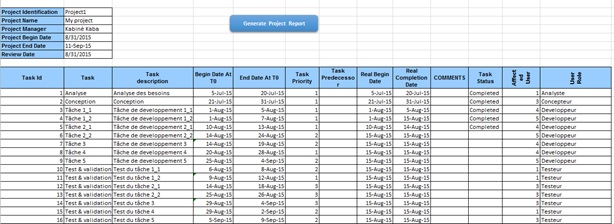
\includegraphics[width=15cm]{template.jpg}
\caption{\label{template}Fichier modèle}
\end{figure}
Le premier bloc (information global sur le projet) contient les champs suivants (Champs en anglais).\\
\begin{table}[h]
\centering
\begin{tabular}{|p{5cm}|m{10cm}|}
\hline Champs & Description \tabularnewline
\hline Project identification & L'identifiant du projet (unique par projet) \tabularnewline
\hline Project Name & Le nom du projet \tabularnewline
\hline Project Manager & Le responsable du projet (chef de projet) \tabularnewline
\hline Project Begin Date & La date de début du projet \tabularnewline
\hline Project End Date & La date de fin du projet \tabularnewline
\hline Review Date & La date de dernière mise à jour du fichier \tabularnewline
\hline
\end{tabular}
\caption{\label{bloc1}Information global sur le projet}
\end{table}
\clearpage
Le second bloc (information sur les tâches requises) contient les champs suivants (Champs en anglais):
\begin{table}[h]
\centering
\begin{tabular}{|p{5cm}|m{10cm}|}
\hline Champs & Description \tabularnewline
\hline Task ID & L'identifiant d'une tâche \tabularnewline
\hline Task & Le nom de la tâche \tabularnewline
\hline Task Description & La description de la tâche (champs libre) \tabularnewline
\hline Begin Date AT T0 & La date de début de la tâche telle que planifiée à T0 (c'est-à-dire au tout début du projet). Ce champ ne doit plus être modifié après le lancement du projet \tabularnewline
\hline End Date At T0 & La date de fin de la tâche telle que planifiée à T0 (c'est-à-dire au tout début du projet). Ce champ ne doit plus être modifié après le lancement du projet. \tabularnewline
\hline Task Priority & La priorité de la tâche. C'est un nombre compris entre 1 et 3 \tabularnewline
\hline Task Predecessor & Permet de définir le lien entre tâche. Dans ce tableau, on ne vise pas à gérer les types de liens en série ou en parallèle, mais juste à définir le lien de dépendance entre différents jalons. \tabularnewline
\hline Real Begin Date & La date réelle de début de la tâche. Ce champ est à modifier en fonction des réalités et de l'avancement du projet.  \tabularnewline
\hline Real Completion Date & La date réelle de fin de la tâche. Ce champ est à modifier en fonction des réalités et de l'avancement du projet \tabularnewline
\hline Comments & Un champ commentaire (champ libre) \tabularnewline
\hline Task status & Le statut de la tâche. Permet de mettre un flag pour savoir si la tâche est finie ou non. \tabularnewline
\hline Affected user & L'identifiant de la ressource associée à la tâche. Concerne les ressources humaines \tabularnewline
\hline User role & Le rôle de la ressource (sa fonction) \tabularnewline
\hline
\end{tabular}
\caption{\label{bloc2}Caractéristiques}
\end{table}
\clearpage
En plus des différents filtres natifs qu'on peut utiliser dans Excel pour filtrer sur les jalons, ce fichier contient également un bouton 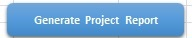
\includegraphics{boutton} qui permet de générer un rapport de performance sur le projet.\\
Ce fichier modèle de base, permet de suivre les jalons, les mettre à jour et à chaque instant pouvoir générer des courbes et des indicateurs (à mettre en place en fonction des besoins) sur le suivi des tâches et leur déviation par rapport à la prévision initiale au début du projet.\\
Dans la section suivante, nous avons détaillé plus en profondeur la partie technique qui nous permet de générer le rapport d'état du projet
\subsubsection*{Le code de génération du rapport de performance}
Le code de génération du rapport de performance est une macro c'est-à-dire qu'il a été développé avec du VBA (Visual Basic For Application) Excel. Architecturalement, ce code est composé des classes et des modules suivants:\\
Une classe \textbf{\textit{C\_Task }}: cette classe représente une tâche. Les attributs de cette classe sont principalement les champs du bloc 2 qui décrivent une tâche dans le fichier modèle.\\
Une classe \textbf{\textit{C\_Projet }}: Cette classe représente le projet dans sa globalité. Elle contient des attributs du bloc 1 qui décrivent le projet de façon global et aussi une liste (collection) de \textbf{\textit{C\_Jalon}}\\
Un module \textbf{\textit{Checker}}:Ce module a trois fonctions principales: 
\begin{itemize}
\item[\tiny{$\blacksquare$}]la première fonction vise à analyser syntaxiquement le fichier modèle, c'est-à-dire s'assurer que les mots clés du fichier sont à la bonne place (champs des jalons et les champs qui décrivent le projet)
\item[\tiny{$\blacksquare$}]la deuxième fonction vise à analyser le type de donnée rentré dans chaque champ et à s'assurer que la valeur saisie est la valeur attendue. La vérification syntaxique du fichier et de la qualité des données rentrées dans les champs garantit une cohérence quant aux données qui sont à traiter.
\item[\tiny{$\blacksquare$}]La troisième fonction vise à vérifier les règles métiers de la gestion du projet. Par exemple, cette partie permettra de vérifier que la date de fin réel d'un jalon ne peut être inférieure à sa date de début etc. C'est vraiment basé sur la cohérence des données qui sont dans le fichier.
\end{itemize}
Un module \textbf{\textit{Reader}}:après la vérification de syntaxe et de cohérence des données, le module Reader permet de lire le fichier Excel et de charger les données dans la classe \textit{C\_Projet}. Ce qui nous permet de gérer des objets de types projets et ainsi bénéficier de la puissance de programmation orientée objet.\\
Un module \textbf{\textit{Mapping}}:afin de ne pas mettre en dure dans le code certains paramètres comme la colonne excel dans laquelle se trouve une valeur et ainsi garantir plus de flexibilité, le module \textit{Mapping} permet de définir l'ensemble des paramètres qui pourraient être modifié demain. Il définit la structure du fichier et permet une utilisation plus propre du fichier.\\
Un module \textbf{\textit{Module Z11}}: ce module contient l'ensemble du code qui permet de générer un rapport de performance.\\
Un module \textbf{\textit{CommonFunctions}}: ce module contient les fonctions communes qui peuvent être utilisées dans les autres modules. On rencontre en autre, les fonctions de conversion en majuscule, les fonctions d'ouverture de l'explorateur pour aller chercher un fichier etc.\\
Pour plus de détails sur le fonctionnement du code, se référer au fichier modèle et ouvrir l'éditeur de texte Visual basic.\\
\begin{figure}[h]
\centering
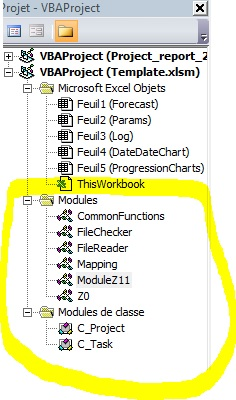
\includegraphics[width=6cm]{vba.jpg}
\caption{\label{struc}Structure des classes et modules}
\end{figure}
\clearpage
\subsubsection*{Développement des modules}
Le module \textbf{\textit{Mapping}} définit la structure du fichier et contient les mots clés et les noms de colonnes. L'image~\ref{mapp} nous donne un extrait de ce module.\\
Le module \textbf{\textit{Mapping}} définit la structure du fichier et contient les mots clés et les noms de colonnes. L'image~\ref{mapp} nous donne un extrait de ce module
\begin{figure}[h]
\centering
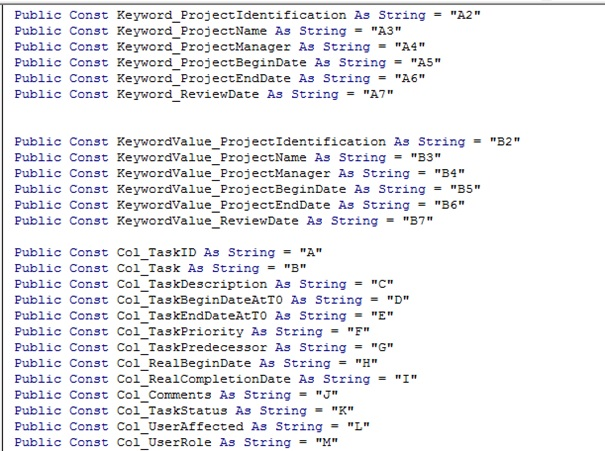
\includegraphics[width=14cm]{mapp.jpg}
\caption{\label{mapp}Mapping module}
\end{figure}
\clearpage
Le module \textbf{\textit{FileChecker}} contient les fonctions suivantes:
\begin{itemize}
\item \textit{VerifSyntaxFile} permet de vérifier la structure du fichier. Retourne vraie si la structure est bonne, et faux dans le cas contraire.
\item \textit{o	VerifiDataFile} permet de vérifier la qualité des données saisies dans le fichier. Retourne vrai si on a les bonnes valeurs dans les champs, et faux s'il y a des champs avec des valeurs incorrectes.
\end{itemize}
Ces deux fonctions sont incluses dans une fonction globale appelée \textit{CheckFile}.\\
Voici une image~\ref{filec} de ce module (Se référer au fichier modèle pour plus de détails)
\clearpage
\begin{figure}[h]
\centering
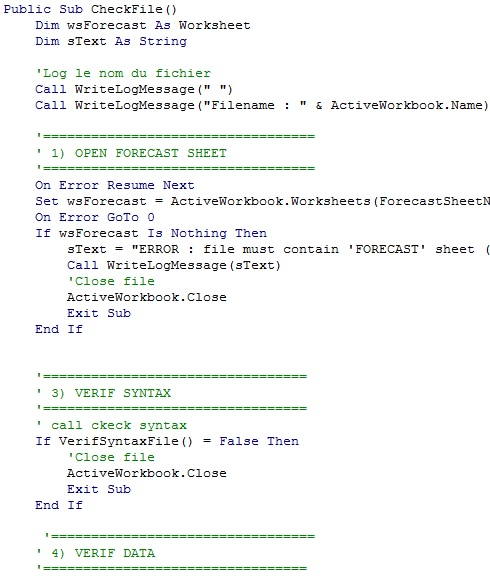
\includegraphics[width=11cm]{filec.jpg}
\caption{\label{filec}FileChecker module}
\end{figure}
Pour des raisons de temps, ce module de vérification n'est pas complètement fini. Beaucoup de cas de vérification restent à implémenter.\\
Le module \textbf{\textit{FileReader}} permet de lire le fichier Excel, transformer les données en un objet \textit{C\_Project} et générer le rapport de performance. Ce module contient les fonctions suivantes:
\begin{itemize}
\item \textbf{\textit{UpdateDATAFromFile}}: permet de lire le fichier modèle et retourne un objet de type \textit{C\_Project}. Voici un extrait de cette fonction~\ref{updff}
\clearpage
\begin{figure}[h]
\centering
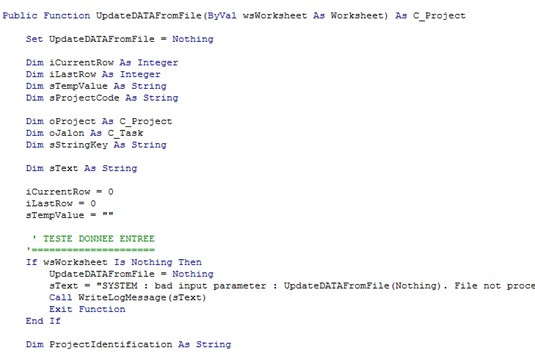
\includegraphics[width=14cm]{updff.jpg}
\caption{\label{updff}Vérification des données d'entrées}
\end{figure}
\item \textbf{\textit{GenerateReportfile}} fait appelle à la fonction \textit{UpdateDataFromFile()} et la fonction \textit{SaveReportFile()} pour générer un rapport de performance.
\end{itemize}
Le module \textbf{\textit{ModuleZ11}} contient les fonctions nécessaires à la génération du rapport. Ces fonctions sont appelées par la fonction \textit{SaveReportingFile}. Ce module contient les fonctionnalités suivantes:
\begin{itemize}
\item \textit{GenerateReportingSheets}: permet de créer dans le rapport de performance les feuilles nécessaires et appelle toutes les autres fonctions pour remplir ces feuilles
\item \textit{WriteDownForectSheetValues}: recopie dans une feuille excel du rapport, les dates nécessaires des tâches lues depuis le fichier modèle
\item \textit{StoreMinAndMaxDate}: permet de détecter et de rajouter la tâche avec la date minimale et la tâche avec la date maximale. Ces dates permettent de définir correctement l'échelle utilisée pour les courbes. Un tri sur les dates est effectué afin de garantir l'ordre
\item \textit{CopyChartsTemplate}: permet de copier dans le fichier des rapports les templates des courbes pour pouvoir mieux tracer dessus (Ces templates sont dans le fichier modèle dans des feuilles cachées)
\item \textit{drawDayDayChart}: permet de tracer la courbe \textit{date-date chart}
\item \textit{drawCumulativeChart}: permet de tracer la courbe \textit{Task Evolution}
\end{itemize}
Le module \textbf{\textit{Commonfunctions}}: contient les fonctions communes utilisées dans toute l'application. Voici un extrait~\ref{comf} de quelques fonctions utilisées dedans.
\begin{figure}[h]
\centering
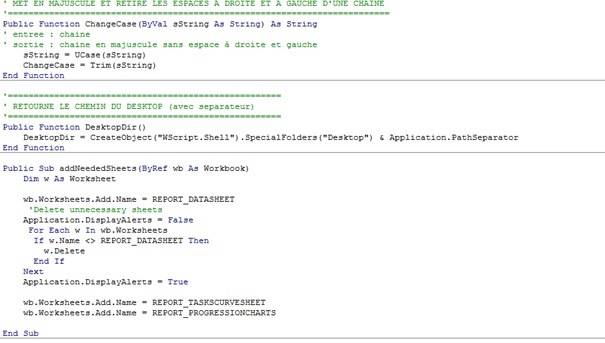
\includegraphics[width=15cm]{comf.jpg}
\caption{\label{comf}Common function}
\end{figure}

\subsection{Application de la solution}
Afin de valider cette deuxième solution, nous l'avons expérimenté sur un projet comportant: une tâche d'analyse, une tâche conception, six tâches de développement des fonctionnalités et six tâches de tests des fonctionnalités développées.
Ce projet a une date de début prévue le 31 août 2015 et une date de fin 11 septembre 2015.
Les tâches d'analyses, conceptions et développement tâche 1\_1 respecte la prévision. Mais à partir de la tâche (tâche 1\_2) on commence à avoir une déviation. En appliquant notre solution sur cet exemple nous obtenons les résultats suivants:
\subsubsection*{Le diagramme Temps-Temps (Date-Date Chart)}
Le diagramme temps-temps est un outil de management de projet. Grâce à une représentation en diagramme temps-temps, il est possible de voir graphiquement l'évolution  au cours du temps des dates prévisionnelles des tâches par rapport aux dates réelles sur un projet. Ce qui nous permet de détecter assez rapidement et de façon visuelle les dérives des tâches par rapport à ce qui était prévu initialement. Par exemple, sur la figure~\ref{graphe1}, nous avons un diagramme temps-temps qui présente graphiquement \textbf{la variation réelle des dates de début des tâches} d'un projet par rapport à ce qui était prévu à l'état initial c'est-à-dire au début du projet.
\begin{figure}[h]
\centering
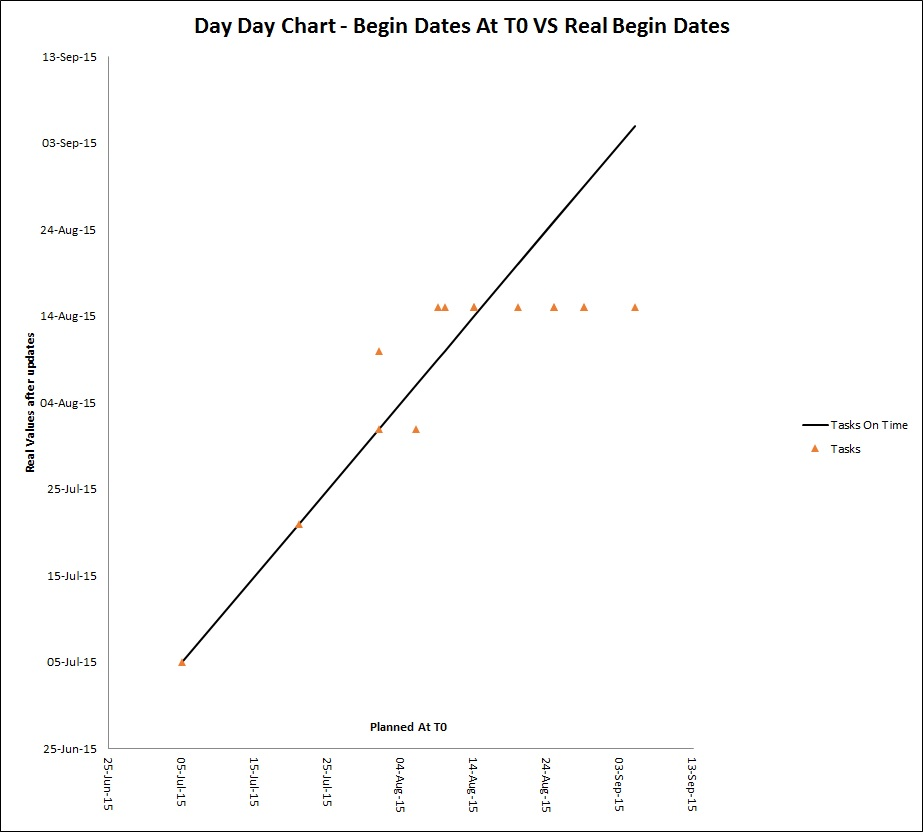
\includegraphics[width=14cm]{graphe1.jpg}
\caption{\label{graphe1}Diagramme Temps-Temps des dates de début des tâches}
\end{figure}
\textbf{Interprétation du diagramme~\ref{graphe1}}
Le diagramme présenté se base sur deux indicateurs des jalons: La date initiale prévue de début des tâches \textit{(Begin date planned at T0)} et la date réelle de début des tâches \textit{(Real begin date)} qui est fréquemment mise à jour. Dans cette figure, l'axe des X (Horizontal) représente le calendrier initial \textit{(dates initiales)} des dates de début des tâches. L'axe des Y (Vertical) représente quant à lui le calendrier des dates de début mises à jour à une période donnée (T).\\
Selon le site \href{http://www.projectplanningoffice.com/}{project planning office}: \og la diagonale d'un tel graphique a toute une signification. Par sa définition mathématique (Y=X), elle correspond à des évènements dont la date prévisionnelle de réalisation ou d'achèvement (Y) et celle du jour où on en fait la prévision (X) sont identiques\fg{}. Dans notre cas, nous pouvons dire que cette diagonale représente la référence \textit{(base line)} des dates de début de nos tâches à la période T0 (Au début du projet) et nous servira à détecter les déviations de dates de début. \\
Les petits triangles (
\includegraphics[width=0.5cm]{triangle}) quant à eux  détermine la dérive des tâches par rapport à la référence. En gros, toutes les tâches qui sont sur la diagonale commencent à la date de début prévue initialement; toutes les tâches qui sont situées au-dessus de la diagonale représentent les tâches qui commencent plus tard que leur date initialement prévue; et toutes les tâches qui sont situées en-dessous de la diagonale représentent les tâches qui commencent plus tôt que leur date initialement prévue.
Pour plus d'information sur les diagrammes temps-temps, vous pouvez vous référer au site de \href{http://www.projectplanningoffice.com/planification-projet-pert-outillage-planificateur-pert-pertificateur/diagramme-dates-dates}{project planning office}.
\textbf{Le même graphique est généré pour les dates de fins des tâches afin de détecter les variations sur les dates de fin (Figure~\ref{graphe2})}.
\begin{figure}[h]
\centering
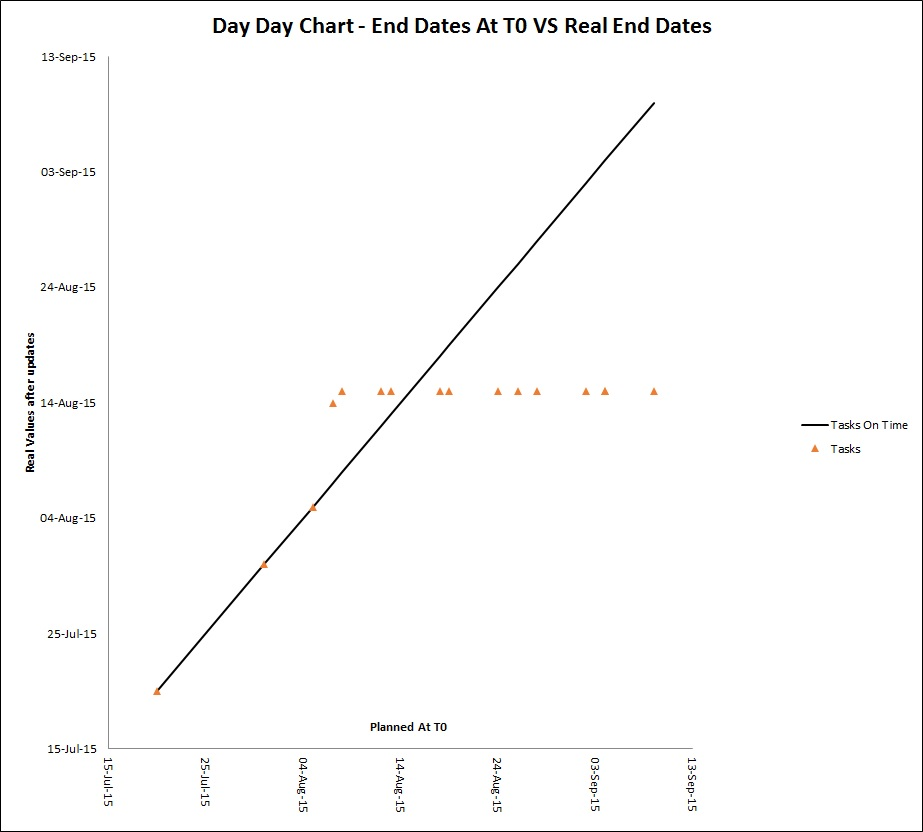
\includegraphics[width=14cm]{graphe2.jpg}
\caption{\label{graphe2}Diagramme Temps-Temps des dates de fins des tâches}
\end{figure}
\subsubsection*{Le diagramme d'évolution des tâches et de comparaison du prévisionnel par rapport au réel}
Ce diagramme est un outil de management de projet et permet de comparer l'évolution des tâches telle que prévue initialement, et l'évolution réelle des tâches après une mise à jour des dates de début de tâche et de fin de tâche.
\begin{figure}[h]
\centering
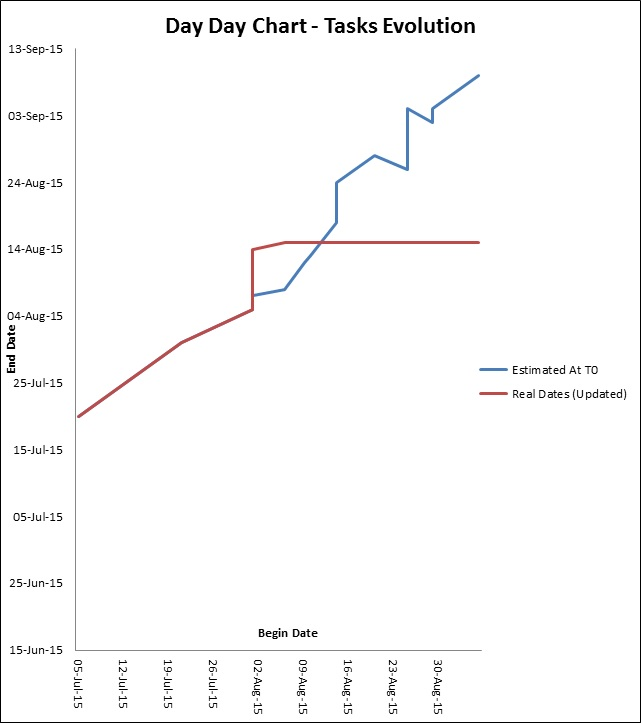
\includegraphics[width=14cm]{graphe3.jpg}
\caption{\label{graphe2}Diagramme d'évolution des tâches}
\end{figure}
\textbf{Interprétation du diagramme~\ref{graphe3}}
Tout comme le diagramme présenté auparavant (Figure~\ref{graphe1}), les axes X et Y de ce graphique~\ref{graphe3} ont des échelles de dates. Sur l'axe des abscisses, on affecte les dates de début des tâches et sur l'axe des ordonnées, on affecte les dates de fin des tâches.\\
Les courbes qui résultent des couples (X, Y) sur ce graphique représentent l'évolution dans le temps des tâches en se basant sur leur date de début et de fin. \\
Dans notre figure, la courbe en bleue représente l'évolution des taches telles que initialement prévues (date de début et de fin initiales) ; et la courbe en rouge représente l'évolution réelle des tâches après mises à jour des dates de début et de fin des taches.\\
En comparant les deux courbes rouge et bleue, on peut interpréter ainsi:
\begin{itemize}
\item[\tiny{$\blacksquare$}]A une date de début d (en regardant l'axe des abscisses X), si le point de la courbe en rouge est au-dessus du point de la courbe en bleue,  ça veut dire qu'il y a un retard sur la réalisation de la tâche par rapport à ce qui était prévu initialement. Si par contre, le point de la courbe en rouge était en dessous du point de la courbe en bleue, ça veut dire qu'on a de l'avance sur la réalisation de tâche par rapport à ce qui était initialement prévu.
\item[\tiny{$\blacksquare$}]A une date de fin f (en regardant l'axe des ordonnées Y), si le point de la courbe en rouge est à droite du point de la courbe en bleue,  ça veut dire qu'on a du retard sur la date de début de la tâche par rapport à ce qui était prévu initialement. Si par contre, le point de la courbe en rouge était à gauche du point de la courbe en bleue, ça veut dire qu'on a de l'avance sur la date de début de la tâche initialement prévue.
\end{itemize}
